\chapter{Preliminary}
In the first section of this chapter we want to recall one of the main objects that appear in this work, namely local systems. In the second section, we provide a concise overview of fundamental algebraic concepts, focusing on Kähler differentials and modules with connections. This serves to formally define differential systems of pure Gaussian type in chapter 3.
~\newline 

We will use the following notation throughout this work:
\begin{itemize}
    \item $\k$ denotes a field. 
    \item $\Vect_\k$ denotes the category of $\k$-vector spaces.
    \item $\Sh_X$ denotes the category of sheaves of $\k$-vector spaces on a topological space $X$.
    \item For a complex vector space $V$ and a topological space $X$ we denote the constant sheaf with fiber $V$ on $X$ by $\underline{V}_X$. Recall that the constant sheaf is obtained through the sheafification of the constant presheaf.
    \item $\C[[t]]$ denotes the ring of formal power series and $\C((t)) = \C[[t]][t^{-1}]$ denotes the ring of formal Laurent series.
    \item $\Dc \coloneqq \C[t]\langle \partial_t \rangle$ denotes the module of differential operators with coefficients in $\C[t]$.
\end{itemize} 

\section{Some sheaf theory}

We begin by recalling some definitions and theorems for local systems and sheaves.

\begin{defi} For a topological space $X$, a \emph{local system} on $X$ is a locally constant sheaf $\Lo$ on $X$. This means that for any point $x \in X$, there is an open neighbourhood $U \subseteq X$, $x \in U$ such that $\Lo_{\vert_U}$ is a constant sheaf.  The category of local systems $\Loc_X$ on $X$ is the full subcategory of $\Sh_X$ where the objects are local systems.
\end{defi}

\begin{comment}
    \begin{lem}
    Let $X$ be a locally connected, topological space. Then $\Loc_X$ is an abelian category.
\end{lem}

\begin{proof}
    Since $\Sh_X$ is an abelian category and $\Loc_X$ is a full subcategory of $\Sh_X$, it suffices to show that $\Loc_X$ is closed under taking kernels and cokernels. Let $\phi: \Lo \to \Lo'$ be a morphism of sheaves between two local systems. Let $x \in X$ be an arbitrary point. Since $\Lo, \Lo'$ are local systems and $X$ is locally connected, there exists an open, connected neighbourhood $U \subseteq X$ of $x$ such that $\Lo_{\vert_U}$ is isomorphic to a constant sheaf $\underline{L}_U$ and $\Lo'_{\vert_U}$ is isomorphic to a constant sheaf $\underline{L'}_U$. We show that $\ker(\phi)_{\vert_U} = \ker(\phi_{\vert_U})$ is isomorphic to the constant sheaf $\underline{\ker \phi_U}_U$. Consider the following diagram with exact rows
    \[
    \begin{xy}
    \xymatrix{
        0  \ar[r] & \ker(\phi_{\vert_U}) \ar@{-->}@/^/[d]  \ar[r] & \Lo_{\vert_U} \ar[r]^{\phi_{\vert_U}} \ar[d]^{\cong}& \Lo'_{\vert_U} \ar[d]^{\cong}\\
        0 \ar[r] & \ker(\psi) \ar@{-->}@/^/_\cong[u]  \ar[r]& \underline{L}_{U} \ar[r]_{\psi} & \underline{L'}_{U}
        }
    \end{xy}
    \]
where $\psi$ is the composition of morphisms so that the diagram commutes. Due to the universal property of the kernel, one gets $\ker(\phi_{\vert_U}) \cong \ker(\psi)$. Lastly we show that $\ker(\psi) \cong \underline{\ker(\phi_U)}_U$. Since $U$ is locally connected, it suffices to show that $\ker(\psi)(V) \cong \underline{\ker(\phi_U)}_U(V)$ holds for any open and connected $V \subseteq U$. 
We have $\Lo_{\vert_U}(U) \cong \underline{L}_U(U) = L = \underline{L}_U(V) \cong \Lo_{\vert_U}(V)$ for any connected, open $V \subseteq U$ and therefore $\ker(\phi_V) \cong \ker(\phi_U)$ which shows that $\ker(\psi)(V) \cong \ker(\phi_V) \cong \underline{\ker(\phi_U)}_U(V)$.
Hence $\ker(\phi)$ is a local system.
\textcolor{red}{Fehlt hier noch etwas?}

For the cokernel we show that the presheaf $\coker(\phi)_{\vert_U} = \coker(\phi_{\vert_U})$ is isomorphic to the constant presheaf $\coker(\phi_U)_U$. Then, using the universal property of the sheafification, we get that the cokernel of $\phi_{\vert_U}$ in $\Sh_X$ is isomorphic to the constant sheaf $\underline{\coker(\phi_U)}_U$. Consider the following diagram in $\PSh_X$
\[
    \begin{xy}
    \xymatrix{
        \Lo_{\vert_U}  \ar[r]^{\phi_{\vert_U}} \ar[d]^{\cong}& \Lo'_{\vert_U}  \ar[d]^{\cong} \ar[r] & \coker(\phi_{\vert_U}) \ar@{-->}@/^/[d] \ar[r] & 0 \\
        \underline{L}_{U} \ar[r]_{\psi} & \underline{L'}_{U}   \ar[r]& \coker(\psi) \ar@{-->}@/^/_\cong[u] \ar[r] & 0
        }
    \end{xy}
    \]
which, using the uinversal property of the cokernel, shows that $\coker(\phi_{\vert_U}) \cong \coker(\psi)$ where $\psi$ is composition of the morphisms so that the diagram commutes. Then for any connected open $V \subseteq U$ we have already seen that $\Lo_{\vert_U}(V) \cong \Lo_{\vert_U}(U)$ and $\Lo'_{\vert_U}(V) \cong \Lo'_{\vert_U}(U)$ and therefore $\phi_U \cong \phi_V$. This shows that
\[
\coker(\psi)(V) = \coker(\psi_V) \cong \coker(\phi_{\vert_U}(V)) = \coker(\phi_V) \cong \coker(\phi_U) = \coker(\phi_U)_U(V)
\]
hence we have $\coker(\psi) \cong \coker(\phi_U)_U$. Thus we get $\coker(\phi_{\vert_U})^\dagger \cong \coker(\psi)^\dagger \cong (\coker(\phi_U)_U)^\dagger = \underline{\coker(\phi_U)}_U$.
\textcolor{red}{Fehlt hier noch etwas?}
\end{proof}
\end{comment}


\begin{prop}[Gluing sheaves]\label{gluedsheaf}
    Let $X$ be a topological space and $\bigcup_{i\in I} U_i = X$ an open covering of $X$. For each $i \in I$, let $\mathcal{F}_i$ be a sheaf on ${U_i}$ and for each pair $(i,j)$ of elements in $I$, let $\phi_{ji}: \mathcal{F}_{i\vert_{U_i\cap U_j}} \to \mathcal{F}_{j\vert_{U_i \cap U_j}}$ be an isomorphism of sheaves such that $\phi_{ii} = \id_{\mathcal{F}_i}$ and on $U_i \cap U_j \cap U_k$ the isomorphisms $\phi_{ik},\phi_{ij}$ and $\phi_{jk}$ satisfy the cocycle relation, i.e.\
    \[
    \phi_{ik} = \phi_{ij} \circ \phi_{jk}.
    \]
    Then, up to isomorphism, there exists a unique sheaf $\mathcal{F}$ on $X$ together with a tuple of isomorphisms $(\psi_i: \mathcal{F}_{\vert_{U_i}} \to \mathcal{F}_i )_{i \in I}$ such that for each pair $(i,j)$ of elements in $I$ \[\phi_{ji} = \psi_j \circ \psi_i^{-1}\] holds on $U_i \cap U_j$.
\end{prop}
\begin{proof} For an open $U \subseteq X$ setting
    \[
    \mathcal{F}(U) \coloneqq \left\{ (s_i)_{i \in I} \in \prod_{i \in I} \mathcal{F}_i(U_i \cap U) ~\Big\vert~ \phi_{ji}\left(s_{i\vert_{U_i \cap U_j}}\right) = s_{j\vert_{U_i \cap U_j}} \text{ for all } i,j \in I \right\}
    \]
    defines a sheaf $\mathcal{F}$ on $X$. Moreover for each $i \in I$ and $U \subseteq U_i$ the morphisms
    \[
    \begin{matrix}
    \psi_i(U) : &\mathcal{F}_{\vert_{U_i}}(U) &\longrightarrow &\mathcal{F}_i(U) \\
    &(s_i)_{i \in I} & \longmapsto & s_i
    \end{matrix}
    \]
    are isomorphisms of vector spaces with inverse
    \[
    \begin{matrix}
    \psi_i(U)^{-1} : &\mathcal{F}_i(U) &\longrightarrow &\mathcal{F}_{\vert_{U_i}}(U). \\
    &s & \longmapsto & (\phi_{ji}(s_{\vert_{U \cap U_j}}))_{j \in I}
    \end{matrix}
    \]
    Remark that $\psi_i^{-1}(U)$ is well-defined because of the cocycle relation. Thus we get isomorphisms of sheaves $(\psi_i)_{i \in I}$. On $U_i \cap U_j$ the relation $\phi_{ji} = \psi_j \psi_i^{-1}$ holds by definition of the isomorphisms $(\psi_i)_{i \in I}$. It is left to prove that the sheaf is unique up to isomorphism. Thus let $\mathcal{G}$ be a sheaf with isomorphisms $(\lambda_i : \mathcal{G}_{\vert U_i} \to \mathcal{F}_i)_{i \in I}$ that satisfy 
    \[
        \phi_{ji} = \lambda_j \lambda_i^{-1}
    \]
    on $U_i \cap U_j$. Then for any $U \subseteq S^1$ define
    \[
    \begin{matrix}
    \alpha(U): &\mathcal{G}(U) &\to &\mathcal{F}(U). \\ 
    & s & \mapsto & (\lambda_{i}(s_{\vert_{U_i\cap U}}))_{i \in I}
    \end{matrix}
    \]
    The morphism $\alpha(U)$ is well-defined as $\phi_{ji} = \lambda_j \lambda_i^{-1}$ on $U_i \cap U_j$ holds. The sheaf axioms of $\mathcal{G}$ show that $\alpha(U)$ is indeed an isomorphism. Hence we get an isomorphism of sheaves $\alpha: \mathcal{G}\to \mathcal{F}$.
\end{proof}

Stokes filtered local systems are local systems on the unit circle $S^1\subseteq \C$, together with a Stokes filtration. So in this thesis we will study objects of $\Loc_{S^1}$. Since we often work with local systems on intervals $I \subsetneq S^1$, we will need the following observations.

\begin{lem}\label{same dimension}
    Let $\mathcal{F}$ be a local system of finite dimensional $\k$-vector spaces on a non-empty, connected topological space $X$. Then all stalks of $\mathcal{F}$ have the same dimension.
\end{lem}

\begin{proof}
    Let $X$ be a non-empty, connected topological space and let $\mathcal{F}$ be a local system on $X$. Then for every point $x \in X$ there is an open subset $U_x \subseteq X$, $x \in U_x$ and a finite dimensional $\k$-vector space $V_x$ with 
    \[
    \mathcal{F}_{\vert_{U_x}} \cong \underline{V_x}_{U_x}.
    \]
    Let $x_o$ be an element in $X$. Set
    \begin{itemize}
        \item $W_1 \coloneqq \{x \in X \mid \dim V_x = \dim V_{x_o}\}$ and
        \item $W_2 \coloneqq \{x \in X \mid \dim V_x \neq \dim V_{x_o}\}$.
    \end{itemize}
    For any point $x \in X$ we have $\mathcal{F}_{\vert_{U_x}} \cong \underline{V_x}_{U_x}$, so for every $x' \in U_x$
    \[
    V_{x'} \cong \left(\mathcal{F}_{\vert_{U_{x'}}}\right)_{x'} = \mathcal{F}_{x'} = \left(\mathcal{F}_{\vert_{U_x}}\right)_{x'} \cong V_x
    \]
    holds. Thus $W_1$ and $W_2$ are open sets. Since $X = W_1 \cup W_2, W_1 \cap W_2 = \varnothing$ and $x_o \in W_1$ we can conclude that $W_2 = \varnothing$, because $X$ is connected. Hence, all stalks of $\mathcal{F}$ have the same dimension.
\end{proof}

\begin{lem}\label{lokalkonstantIntervall}
    Let $\mathcal{F}$ be a local system on a closed interval $[a,b] \subseteq \R$. Then $\mathcal{F}$ is a constant sheaf on $[a,b]$.
\end{lem}

\begin{rem}
    More generally, one can show that a local system on a contractible space $X$ is a constant sheaf on $X$. However, as we specifically require the statement for intervals, proving (\ref{lokalkonstantIntervall}) suffices.
\end{rem}

\begin{proof}
    Let $\mathcal{F}$ be an object in $\Loc_{[a,b]}$. Then for every $x \in [a,b]$ there is an open neighbourhood $U_x\subseteq [a,b], x \in U_x$ so that $\mathcal{F}_{\vert_{U_x}}$ is constant, i.e.\ there exists a finite dimensional $\k$-vector space $V_x$ and an isomorphism of sheaves $\phi_x: \mathcal{F}_{\vert_{U_x}} \to \underline{V_x}_{U_x}$. Since $[a,b]$ is connected, we can set $V \coloneqq V_a$ and assume $\mathcal{F}_{\vert_{U_x}} \cong \underline{V}_{U_x}$ for all points $x \in [a,b]$ by using lemma (\ref{same dimension}).
    $\bigcup_{x \in [a,b]} U_x$ is an open covering of $[a,b]$ and by compactness of the closed interval we find a finite subcover $[a,b]=\bigcup_{i=1}^n U_{x_i}$. By refining and renumbering the cover if necessary, we can assume without loss of generality that the subcover satisfies the following properties:
    \begin{enumerate}
        \item Any open set $U_{x_i}$ of the subcover is connected.
        \item There are no triple intersections, namely for three pairwise different indices $i,j,k \in \{1, \dots, n\}$ we have $U_{x_i}\cap U_{x_j} \cap U_{x_k} = \varnothing$.
        \item For $i, j \in \{1, \dots n\}$ we have $x_i < x_j$ if $i < j$.
        \item For $i \in \{1, \dots, n-1\}$ we have $U_{x_i} \cap U_{x_{i+1}} \neq \varnothing$.
    \end{enumerate}

\begin{figure}[h!]
    \centering    
    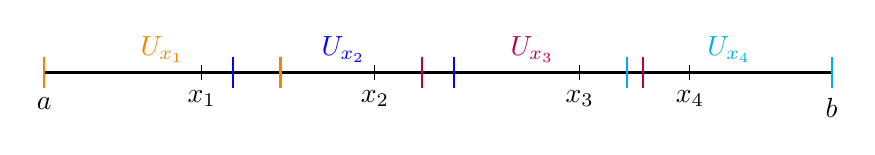
\begin{tikzpicture}[scale=2]
    \def\a{0}
    \def\b{5}

    \def\xa{1}
    \def\xb{2.1}
    \def\xc{3.4}
    \def\xd{4.1}

    \def\xaj{1.5}
    \def\xbi{1.2}
    \def\xbj{2.6}
    \def\xci{2.4}
    \def\xcj{3.8}
    \def\xdi{3.7}
    \def\xdj{4.3}
    
    \draw[thick] (\a,0) -- (\b,0);
    \draw (\a,0.1) -- (\a,-0.1) node[below] {$a$};
    \draw (\b,0.1) -- (\b,-0.1) node[below] {$b$};
    \draw (\xa,0.05) -- (\xa,-0.05) node[below] {$x_1$};
    \draw (\xb,0.05) -- (\xb,-0.05) node[below] {$x_2$};
    \draw (\xc,0.05) -- (\xc,-0.05) node[below] {$x_3$};
    \draw (\xd,0.05) -- (\xd,-0.05) node[below] {$x_4$};

    \node[inner sep=0pt] (a) at (\a,0) {};
    \node[inner sep=0pt] (xaj) at (\xaj,0) {};
    \node[inner sep=0pt] (xbi) at (\xbi,0) {};
    \node[inner sep=0pt] (xbj) at (\xbj,0) {};
    \node[inner sep=0pt] (xci) at (\xci,0) {};
    \node[inner sep=0pt] (xcj) at (\xcj,0) {};
    \node[inner sep=0pt] (xdi) at (\xdi,0) {};
    \node[inner sep=0pt] (b) at (\b,0) {};

    \draw[black] (a) -- (xaj) node[midway,above,text=orange] {$U_{x_1}$};
    \draw[black] (xbi) -- (xbj) node[midway,above,text=blue] {$U_{x_2}$};
    \draw[black] (xci) -- (xcj) node[midway,above,text=purple] {$U_{x_3}$};
    \draw[black] (xdi) -- (b) node[midway,above,text=cyan] {$U_{x_4}$};

    \draw[orange, thick] (\a, 0.1) -- (\a, -0.1);
    \draw[orange, thick] (\xaj, 0.1) -- (\xaj, -0.1);
    \draw[blue, thick] (\xbi, 0.1) -- (\xbi, -0.1);
    \draw[blue, thick] (\xbj, 0.1) -- (\xbj, -0.1);
    \draw[purple, thick] (\xci, 0.1) -- (\xci, -0.1);
    \draw[purple, thick] (\xcj, 0.1) -- (\xcj, -0.1);
    \draw[cyan, thick] (\xdi, 0.1) -- (\xdi, -0.1);
    \draw[cyan, thick] (\b, 0.1) -- (\b, -0.1);
    \end{tikzpicture}
    
    \caption{Sketch of an example subcover of the interval $[a,b]$ satisfying the previous properties.}
\end{figure}

     Using the notation $U_{ij} \coloneqq U_{x_i} \cap U_{x_j}$ we get the following diagram on $U_{12}$:

    \[
        \begin{tikzcd}[row sep=1.5cm, column sep=2cm]
         & \mathcal{F}_{\vert_{U_{x_1}}} \arrow[d, "(\bullet)_{\vert_{U_{12}}}"] \arrow[ddd, swap, "\phi_{x_1}", bend right=40] & \mathcal{F}_{\vert_{U_{x_2}}} \arrow[d, swap, "(\bullet)_{\vert_{U_{12}}}"] \arrow[ddd, "\phi_{x_2}", bend left=40] & \\
        & \mathcal{F}_{\vert_{U_{12}}} \arrow[r, swap, "\id_{\mathcal{F}_{\vert_{U_{12}}}}"] \arrow[d, "\phi_{x_1\vert_{U_{12}}}"] &  \mathcal{F}_{\vert_{U_{12}}} \arrow[d, swap, "\phi_{x_2\vert_{U_{12}}}"]& \\
        & \underline{V}_{U_{12}} \arrow[r, "\lambda"] & \underline{V}_{U_{12}} & \\
        & \underline{V}_{U_{x_1}} \arrow[u, swap, "(\bullet)_{\vert_{U_{12}}}"] & \underline{V}_{U_{x_2}} \arrow[u, "(\bullet)_{\vert_{U_{12}}}"] &
        \end{tikzcd}
    \]

Here $\lambda$ is given by $\phi_{x_2\vert_{U_{12}}} \circ \phi_{x_1\vert_{U_{12}}}^{-1}$. Since $\mathcal{F}_{\vert_{U_{x_i}}}$ is constant, the restriction maps $(\bullet)_{\vert_{U_{ij}}}$ are isomorphisms. Thus we can change $\phi_{x_2}: \mathcal{F}_{\vert_{U_{x_2}}} \to \underline{V}_{U_{x_2}}$ by taking the composition with an automorphism $\alpha_2: \underline{V}_{U_{x_2}} \to \underline{V}_{U_{x_2}}$ in such way that we get $(\alpha_2 \phi_{x_2})_{\vert_{U_{12}}} = \phi_{x_1\vert_{U_{12}}}$. In particular, we obtain $\lambda =\id_{\underline{V}_{U_{12}}}$. We set $\tilde{\phi}_{x_2} \coloneqq \alpha_2 \circ \phi_{x_2}$.

Using (\ref{gluedsheaf}), $\mathcal{F}_{\vert_{U_{x_1}}}$,  $\mathcal{F}_{\vert_{U_{x_2}}}$ glue together to $\mathcal{F}_{\vert_{U_{x_1} \cup U_{x_2}}}$. Moreover, since $\underline{V}_{U_{x_1} \cup U_{x_2}}$ together with $\phi_{x_1}^{-1}: \underline{V}_{U_{x_1}} \to \mathcal{F}_{\vert U_{x_1}}$ and $\tilde{\phi}_{x_2}^{-1}: \underline{V}_{U_{x_2}} \to \mathcal{F}_{\vert U_{x_2}}$ fulfill 
\[
\id_{\mathcal{F}_{\vert_{U_{12}}}} = \tilde{\phi}_{x_2\vert_{U_{12}}}^{-1}\phi_{x_1\vert_{U_{12}}},
\]
we get an isomorphism $\mathcal{F}_{\vert_{U_{x_1} \cup U_{x_2}}} \to \underline{V}_{U_{x_1} \cup U_{x_2}}$ by application of lemma (\ref{gluedsheaf}). We repeat this successively for $\mathcal{F}_{\vert_{ U_1 \cup \dots \cup U_{x_i}}}$ and $\mathcal{F}_{\vert_{U_{x_{i+1}}}}$ until we finally get 
$\mathcal{F} \cong \underline{V}_{[a,b]}$.
\end{proof}

Using lemma (\ref{lokalkonstantIntervall}), it becomes apparent that a local system $\Lo$ defined on $S^1$ and restricted to an interval $I\subsetneq S^1$ is a constant sheaf if its closure is not equal to $S^1$.


\begin{rem}
    Local systems on $S^1$ can also be studied from a different point of view using the following theorem: 
\begin{thm}\label{monodromy}
Let $X$ be a connected and locally simply connected topological space, and $x$ a point in $X$. The category $\Loc_X$ is equivalent to the category of finite dimensional representations of $\pi_1(X,x)$.
\end{thm}
\begin{proof}
    See \cite{szamuely_2009}, Corollary 2.6.2.
\end{proof}
 The theorem shows that giving a local system of dimension $n$ on $S^1$ is equivalent to giving a homomorphism of groups $\Z \cong \pi_1(S^1,1) \to \GL(\C^n)$, i.e.\ an element in $\GL(\C^n)$. This element is called the \emph{monodromy representation} of the local system. In the following we will not need this equivalence of categories, but it could be beneficial to keep it in mind.
\end{rem}


\section{Kähler differentials and modules with connections}

In this section we recall the module of Kähler differentials for algebras over some commutative ring $R$ with unit in order to define modules with connections afterwards. This is necessary to give the formal definition of differential system of pure Gaussian type in the next chapter. For more details see chapter 4 in \cite{LinAlg}. 

\begin{defi}
Let $R$ be a commutative ring with unit and $A$ be an $R$-algebra. A \emph{derivation} from $A$ to a left $A$-module $M$ is an $R$-linear mapping $D:A \to M$ that fulfills the Leibnitz rule, namely \[D(fg) = fD(g) + gD(f)\] holds for all $f,g \in A$.   
The set of derivations from $A$ to $M$ is denoted by $\Der_R(A,M)$.
\end{defi}
 One can check that $\Der_R(A,M)$ is an $A$-module.


\begin{defi} Let $R$ be a commutative ring with unit and let $A$ be a commutative $R$-algebra.
    The \emph{module of Kähler differentials of $A$ over $R$}, denoted by $\Omega_{A/R}$, is an $A$-module together with a derivation $d_{A/R} \in \Der_R(A, \Omega_{A/R})$, which satisfies the following universal property: For any $A$-module $M$ and any derivation $D\in \Der_R(A,M)$ there is a unique $A$-module homomorphism $\phi: \Omega_{A/R}^1 \to M$ with $D= \phi \circ d_{A/R}$, i.e.\ the following diagram commutes:
    \[
    \begin{xy}
    \xymatrix{
    A \ar[r]^{d_{A/R}} \ar[rd]_D & \Omega_{A/R} \ar@{-->}[d]^\phi \\ 
    & M 
    }
    \end{xy}
    \]
\end{defi}

\begin{rem}
    For a commutative $R$-algebra $A$ one can check that there always exists the module of Kähler differentials $(\Omega_{A/R}, d_{A/R})$. For details see (\cite{LinAlg}, 4.2.1. and  4.2.2). 
\end{rem}


\begin{ex}\label{KaehlerBsp}
For $A = \k[x_1,\dots,x_n]$ one has $(\Omega_{A/\k}, d_{A/\k}) = (\bigoplus_{i=1}^n A \diff{x_i}, d_{A/\k})$ with 
\[
\begin{matrix}
    d_{A/\k}: & A & \to & \bigoplus_{i=1}^n A \diff{x_i} \\
    & f & \mapsto & (\frac{\partial f}{\partial x_i} \diff{x_i})_{i \in \{1, \dots n\}}
\end{matrix}
\] as $(\bigoplus_{i=1}^n A \diff{x_i}, d_{A/\k})$ satisfies the universal property. Analogously for the ring of formal power series $A = \k[[x]]$ one has $\Omega_{A/\k} = \k[[x]]\diff{x}$ with $d_{A/\k}(f(x)) = \frac{\partial f}{\partial x}(x) \diff{x}$ where $\frac{\partial f}{\partial x}(x)$ is the formal differentiation of the formal power series $f$.
\end{ex}

\begin{lem}\label{kaehlerloca} The module of Kähler differentials is compatible with localization, i.e.\ for an $R$-algebra $A$ and a multiplicative system $S$ in $A$
\[
\Omega_{S^{-1}A/R} = S^{-1}\Omega_{A/R}
\]
holds.
\end{lem}
\begin{proof}
    See \cite{Hart}, proposition 8.2A.
\end{proof}

\begin{defi} Let $A$ be a commutative $\k$-algebra and $(\Omega_{A/\k}^1, d_{A/\k})$ the module of Kähler differentials of $A$ over $\k$. An \emph{$A$-module with connection} is an $A$-module $M$ together with a $\k$-linear connection, i.e.\ a $\k$-linear morphism 
\[
\nabla: M \to \Omega_{A/\k}^1 \otimes_A M   
\]
satisfying the Leibnitz rule, namely
\[\nabla(am) = d_{A/\k}(a) \otimes m + a \nabla(m)\]
holds for all $a \in A$ and $m \in M$. 

Let $(M,\nabla_M), (N,\nabla_N)$ be two $A$-modules with connections. Then an $A$-linear morphism $\phi: M \to N$ is called a \emph{morphism of $A$-modules with connections} if $(\id \otimes \phi) \circ \nabla_M = \nabla_N \circ \phi$. 
We denote the category of $A$-modules with connection by $\Conn(A)$.
\end{defi} 

\begin{ex}\label{C-con}
With example (\ref{KaehlerBsp}) we get $(\Omega_{\C[t]/\C}, d_{\C[t]/\C}) = (\C[t] \diff t, d_{\C[t]/\C}: f \mapsto \frac{\partial f}{\partial t}\diff t)$. Thus a $\C[t]$-module with connection is a $\C[t]$-module $M$ together with a $\C$-linear morphism
\[\nabla: M \to \C[t]\diff{t} \otimes_{\C[t]} M\]
that satisfies the Leibnitz rule
\[\nabla(fm) = d_{\C[t]/\C}(f) \otimes m + f \nabla(m) = \frac{\partial f}{\partial t}\diff{t} \otimes m + f \nabla(m).\]
\end{ex}

\begin{ex}
    A $\C((t))$-vector space $\mathcal{M}$ of finite dimension with a connection $\nabla: \mathcal{M} \to \Omega_{\C((t))/\C} \otimes_{\C((t))} \mathcal{M}$ is also called a \emph{meromorphic connection}.
\end{ex}


After we have clarified foundational concepts, we can apply them in the following chapter to get to the definitions of differential systems of Gaussian type and Stokes filtered local systems. Moreover we will link both concepts in the end of the next chapter using a Riemann-Hilbert correspondence.